\lab{Classification Trees}{Classification Trees}
\objective{Understand how to build a classification tree and use it to predict survival of Titanic passengers.}

Classification trees are a class of decision trees, and are used in a wide variety of settings where labeled training data is available, and where the desired outcome is a model which is able to accurately assign labels to unlabeled data. We assume that each sample $d$ has $P$ attributes, which can be real-valued or categorical, and that each sample belongs to some class $k$, where there are $K$ classes. The tree is composed of many \emph{nodes}, which represent a decision point (i.e. a question is asked about the sample which has a boolean response). If the response is \li{True}, then the sample is ``pushed'' down the tree to the left child node. If the response is \li{False}, then the sample is ``pushed'' down the tree to the right child node. A \emph{leaf} node is a node that has no child node, i.e. it is the end of the line and there is not a question asked.  Each leaf has a classification assigned to it, and an unlabeled sample is labeled with that classification upon arrival at the leaf node.

How do we train a classification tree? We start with a labeled data set $D$ and choose the best attribute $p$ and value $x$ by which to \emph{split} the data. We have now partitioned $D$ into two sets, which we may then split as well. We continue in this manner until some stopping criterion is met (often a maximum depth of the tree). To formalize this, we need several definitions.

\begin{definition}
Let $D$ be a data set with $K$ different classes. Let $N_{k}$ be the number of samples labeled class $k$ for each $1 \leq k \leq K$, and let $f_{k} = \frac{N_{k}}{N}$ where $N$ is the total number of samples in $D$. We define the \emph{Gini impurity} to be 
\begin{equation*}
G(D) = 1 - \sum_{k=1}^{K} f_{k}^{2}.
\end{equation*}
\end{definition}

\begin{problem}
Write a function that accepts a list of class assignments and a list of all the $K$ possible classes, and computes the Gini impurity.
\end{problem}

\begin{definition}
We define the \emph{split} $s_{D}(p,x)$ of the data set $D$ on attribute $p$ using value $x$, to be a partition $D_{1},D_{2}$ such that 
\begin{enumerate}
	\item $d_{p} \leq x$ for all $d \in D_{1}$ and $d_{p} > x$ for all $d \in D_{2}$, where $d_{p}$ is the value of attribute $p$ in $d$, assuming real values; or \\
	\item $d_{p} = x$ for all $d \in D_{1}$ and $d_{p} \neq x$ for all $d \in D_{2}$, where $d_{p}$ is the value of attribute $p$ in $d$, assuming categorical values.
\end{enumerate}
\end{definition}

\begin{problem}
Write a function that computes the split of a data set for a given variable $p$ and given value $x$. It should return the partitioned data set, as well as the partitioned class labels.
\end{problem}

\begin{definition}
Let $s_{D}(p,x) = D_{1},D_{2}$ be a split. We define the \emph{information gain} of this split to be 
\begin{equation*}
I(s_{D}(p,x)) = G(D) - \sum_{i=1}^{2} \frac{\abs{D_{i}}}{\abs{D}} \cdot G(D_{i})
\end{equation*}
\end{definition}

\begin{problem}
Write a function that computes the information gain for the split of a data set for a given variable $p$, value $x$.
\end{problem}

We define the optimal split of a data set to be
\begin{equation*}
s_{D}^{*} = s_{D}(p^{*}, x^{*}),
\end{equation*}
where 
\begin{equation*}
p^{*}, x^{*} = \text{argmax}_{p,x} I(s_{D}(p,x)).
\end{equation*}
From this partition, we create two child nodes, assigning the left child node data set $D_{1}$, and right child node data set $D_{2}$.

\begin{problem}
Write a function that computes the optimal split of a data set. You may need to separate this into two tasks: finding the optimal split for each attribute $p$, and then choosing the optimal split over all the attributes.
\end{problem}

Let's put all of this together to create the full classification tree.

\begin{problem}
Write a class called \li{Node} that creates and trains a classification tree. It should accept a training data set $D$, class labels $y$, current depth (which when initialized should be $1$), some maximum depth which is greater than $1$, and some tolerance for the Gini impurity (say $0.2$). Use recursion to build the tree, i.e. after determining the optimal split, create two new nodes (\li{leftchild} and \li{rightchild}), with incremented depth. If the depth equals the maximum depth or the Gini impurity for a node is less than the tolerance, assign the majority label to the node and do not split further.
\end{problem}

\begin{problem}
Write a method for the class \li{Node} that prints out the tree structure. For each node it should show which attribute $p$ and value $x$ provide the optimal split, and for the leaf nodes, it should show the assigned label. You may use your own creativity for how to display this.
\end{problem}

\begin{problem}
Write a method for the class \emph{Node} that assigns the class label for a new sample. You will probably have to make this method recursive also.
\end{problem}

We would like to test our classifier on a real data set. Provided for you is a data set on about $1000$ passengers aboard the Titanic. We would like to predict their survival or death depending on several attributes: class ($1^{st}, 2^{nd},$ or $3^{rd}$), gender (male or female), and age.

\begin{problem}
Using the Titanic data set, train a classification tree with a maximum depth of $10$ nodes and Gini impurity tolerance $.1$, and predict labels for the test set. What is your misclassification rate? Print out the tree structure. Is it what you expected? Was there any optimal split which surprised you?
\end{problem}

The free parameters which we can vary are the maximum depth and the Gini impurity tolerance. Higher values for the maximum depth creates more refined, specific trees, as does a smaller Gini impurity tolerance. In this case, we are making the classifier more \emph{complex}. As such, it will perform better on the data on which it is trained (it has learned the training data well), but perform worse on new, test data (it is not very generalizable). Keeping the Gini impurity tolerance at $0.1$ and increasing the maximum depth yields the following interesting misclassification curves. What is the take away message?

\begin{figure}
\centering
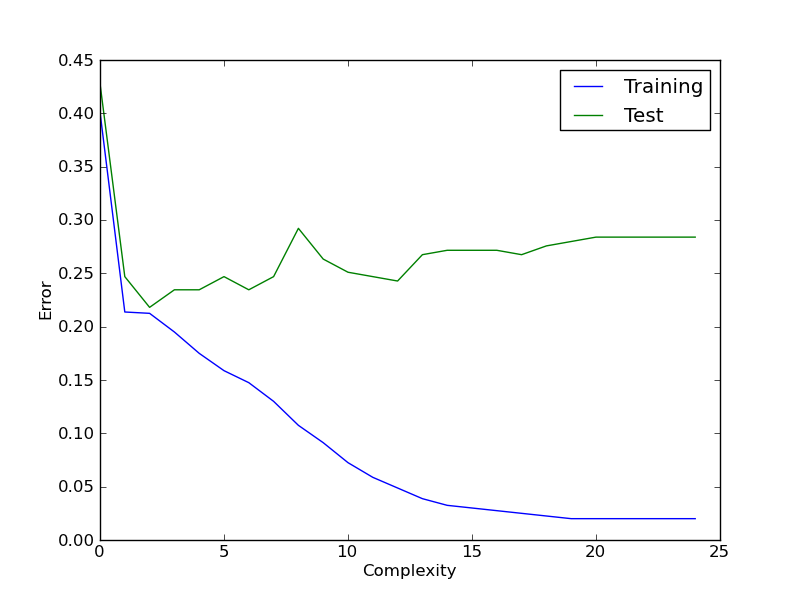
\includegraphics[width=\textwidth]{complexity.png}
\caption{Misclassification rate on training data and test data with increasing complexity.}
\end{figure}
